\documentclass{article}
\usepackage[utf8]{inputenc}
\usepackage{amsmath}
\usepackage{amsfonts}
\usepackage{amssymb}
\usepackage{graphicx}
\usepackage{tikz}
\usepackage{enumitem}
\usepackage{listings}
\usepackage{xcolor}
\usepackage{hyperref}
\usepackage{geometry}
\usepackage{fancyhdr}
\usepackage{multicol}

\geometry{margin=1in}
\pagestyle{fancy}
\fancyhf{}
\rhead{Lecture 2: Universal Tool Calling Demo}

\cfoot{\thepage}

\definecolor{codegray}{gray}{0.95}
\definecolor{keyword}{RGB}{0,0,255}
\definecolor{string}{RGB}{163,21,21}
\definecolor{comment}{RGB}{0,128,0}

\lstset{
    backgroundcolor=\color{codegray},
    basicstyle=\ttfamily\footnotesize,
    breaklines=true,
    captionpos=b,
    commentstyle=\color{comment},
    frame=single,
    keywordstyle=\color{keyword},
    language=Python,
    numbers=left,
    numbersep=5pt,
    showstringspaces=false,
    stringstyle=\color{string},
    tabsize=4
}

\title{Lecture 2: Universal Tool Calling Demo\\AI Agent Development with Multi-Backend LLM Integration}
\author{(Jack) Yansong Li}
\date{\today}

\begin{document}

\maketitle

\section{Introduction and Course Overview}

\subsection{Learning Objectives}

By the end of this lecture, students will be able to:

\begin{enumerate}[label=\arabic*.]
    \item Understand the architecture of universal AI agents with automatic backend selection
    \item Implement OpenAI-compatible tool calling mechanisms with proper error handling
    \item Design and develop streaming architectures for real-time AI applications
    \item Build cross-platform compatible AI systems with intelligent fallback strategies
    \item Create extensible tool registries with dynamic registration capabilities
    \item Apply modern software engineering patterns to AI agent development
    \item Deploy and test AI agents across different hardware configurations
\end{enumerate}

\subsection{Project Overview}

The Universal Tool Calling Demo is a sophisticated educational project that demonstrates advanced LLM tool calling functionality across multiple platforms. This project serves as a comprehensive example of modern AI agent development, showcasing:

\begin{itemize}
    \item \textbf{Automatic Backend Selection}: Intelligent detection of system capabilities and optimal backend routing
    \item \textbf{OpenAI-Compatible Tool Calling}: Standard function calling format with extensible tool registry
    \item \textbf{Real-time Streaming}: Multi-phase streaming with visual feedback for different content types
    \item \textbf{Cross-Platform Compatibility}: Universal deployment across Windows, macOS, and Linux
    \item \textbf{Modern Development Practices}: Comprehensive testing, configuration management, and deployment strategies
\end{itemize}

\subsection{Technology Stack}
See Table~\ref{table:tech-stack}.

\begin{table}[ht]
\centering
\begin{tabular}{|l|l|l|}
\hline
\textbf{Component} & \textbf{Technology} & \textbf{Purpose} \\
\hline
LLM Inference & vLLM (>=0.6.0) & High-performance GPU inference \\
Local Inference & Ollama (>=0.1.0) & CPU-based local inference \\
API Framework & FastAPI + Uvicorn & vLLM server management \\
Package Management & UV & Fast, reliable dependency management \\
Model & Qwen3-0.6B & Tool-optimized language model \\
Testing & pytest + coverage & Comprehensive test suite \\
Configuration & python-dotenv & Environment-based configuration \\
\hline
\end{tabular}
\caption{Technology Stack Overview}
\label{table:tech-stack}
\end{table}

\section{Architecture and Design Patterns}

\subsection{High-Level Architecture}

The system employs a \textbf{Universal Agent Pattern} with intelligent backend selection:

\begin{center}
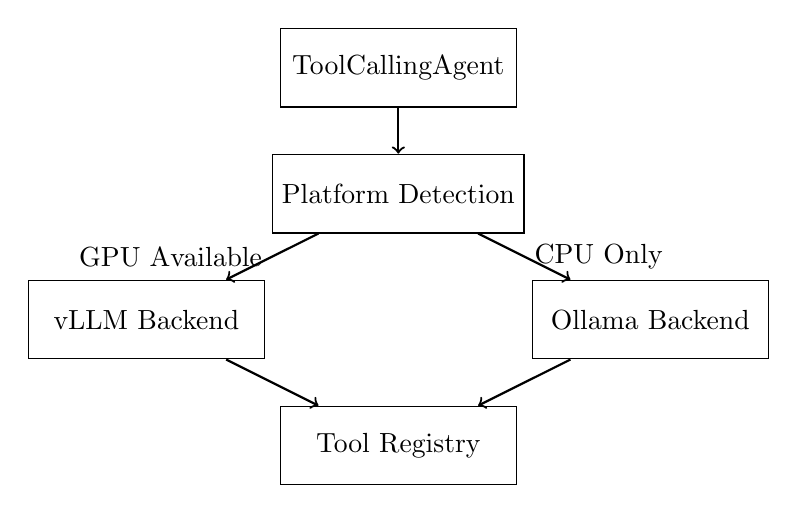
\begin{tikzpicture}[scale=0.8]
\node[rectangle, draw, minimum width=3cm, minimum height=1cm] (main) at (0,0) {ToolCallingAgent};
\node[rectangle, draw, minimum width=3cm, minimum height=1cm] (detect) at (0,-2) {Platform Detection};
\node[rectangle, draw, minimum width=3cm, minimum height=1cm] (vllm) at (-4,-4) {vLLM Backend};
\node[rectangle, draw, minimum width=3cm, minimum height=1cm] (ollama) at (4,-4) {Ollama Backend};
\node[rectangle, draw, minimum width=3cm, minimum height=1cm] (tools) at (0,-6) {Tool Registry};

\draw[->, thick] (main) -- (detect);
\draw[->, thick] (detect) -- node[left] {GPU Available} (vllm);
\draw[->, thick] (detect) -- node[right] {CPU Only} (ollama);
\draw[->, thick] (vllm) -- (tools);
\draw[->, thick] (ollama) -- (tools);
\end{tikzpicture}
\end{center}

\subsection{Core Design Patterns}

\subsubsection{Strategy Pattern: Backend Selection}

The system intelligently selects the optimal backend based on platform capabilities:

\begin{lstlisting}[caption=Backend Selection Strategy]
class ToolCallingAgent:
    def _detect_best_backend(self) -> str:
        """Intelligent backend selection based on system capabilities."""
        system = platform.system()

        # macOS - Always use Ollama for optimal compatibility
        if system == "Darwin":
            return "ollama"

        # Windows/Linux - Check for CUDA availability
        if torch.cuda.is_available():
            gpu_memory = torch.cuda.get_device_properties(0).total_memory
            if gpu_memory >= 4 * 1024**3:  # 4GB minimum
                return "vllm"

        # Fallback to Ollama for CPU systems
        return "ollama"
\end{lstlisting}

\subsubsection{Factory Pattern: Agent Creation}

Automatic agent initialization based on detected capabilities:




\begin{lstlisting}[caption=Factory Pattern Implementation]
def _initialize_backend(self):
    """Factory method for backend initialization."""
    if self.backend_type == "vllm":
        self._init_vllm()
    elif self.backend_type == "ollama":
        self._init_ollama()
    else:
        raise ValueError(f"Unsupported backend: {self.backend_type}")
\end{lstlisting}

\subsubsection{Observer Pattern: Streaming Architecture}

Real-time streaming with multiple content types:

\begin{lstlisting}[caption=Streaming Observer Pattern]
def chat_stream(self, message: str, use_tools: bool = True):
    """Streaming chat with multiple chunk types."""
    for chunk in self._process_stream(message):
        chunk_type = chunk.get("type")
        content = chunk.get("content", "")

        if chunk_type == "thinking":
            yield {"type": "thinking", "content": content}  # Gray text
        elif chunk_type == "tool_call":
            yield {"type": "tool_call", "content": content}  # Blue notification
        elif chunk_type == "tool_result":
            yield {"type": "tool_result", "content": content}  # Green result
        elif chunk_type == "content":
            yield {"type": "content", "content": content}  # Final response
\end{lstlisting}

\subsubsection{Registry Pattern: Tool Management}

Extensible tool system with dynamic registration:

\begin{lstlisting}[caption=Tool Registry Pattern]
class ToolRegistry:
    def __init__(self):
        self.tools = {}
        self._register_builtin_tools()

    def register_tool(self, name: str, function: callable,
                     description: str, parameters: Dict):
        """Register a new tool with OpenAI-compatible schema."""
        self.tools[name] = {
            "function": function,
            "description": description,
            "parameters": parameters
        }

    def execute_tool(self, name: str, arguments: Dict) -> str:
        """Execute a registered tool with error handling."""
        if name not in self.tools:
            return json.dumps({"error": f"Tool {name} not found"})

        try:
            tool_func = self.tools[name]["function"]
            result = tool_func(**arguments)
            return json.dumps({"success": True, "result": result})
        except Exception as e:
            return json.dumps({
                "success": False,
                "error": str(e),
                "traceback": traceback.format_exc()
            })
\end{lstlisting}

\section{Tool Calling Mechanisms}

\subsection{OpenAI-Compatible Function Calling}

The system implements the standard OpenAI function calling format:

\begin{lstlisting}[caption=Function Calling Schema]
{
  "tool_calls": [{
    "id": "call_123",
    "type": "function",
    "function": {
      "name": "get_weather",
      "arguments": {
        "location": "Tokyo, Japan",
        "unit": "celsius"
      }
    }
  }]
}
\end{lstlisting}

\subsection{ReAct Loop Implementation}

The ReAct (Reasoning + Acting) pattern enables multi-step problem solving:

\begin{lstlisting}[caption=ReAct Loop Implementation]
def _process_with_tools(self, message: str, max_iterations: int = 10):
    """Multi-step reasoning with tool execution."""
    iteration = 0

    while iteration < max_iterations:
        # Get model response
        response = self._get_model_response(message)

        # Parse tool calls from response
        tool_calls = self._parse_tool_calls(response)

        if not tool_calls:
            # No tools needed, return final response
            return response

        # Execute tools and collect results
        tool_results = []
        for tool_call in tool_calls:
            result = self.tool_registry.execute_tool(
                tool_call["name"],
                tool_call["arguments"]
            )
            tool_results.append({
                "tool_call_id": tool_call["id"],
                "result": result
            })

        # Add results to conversation history
        self.conversation_history.extend(tool_results)

        iteration += 1

    return "Maximum iterations reached"
\end{lstlisting}

\subsection{Built-in Tools Analysis}

\subsubsection{Weather Tool}

Real-time weather data retrieval with location parsing:

\begin{lstlisting}[caption=Weather Tool Implementation]
def get_current_temperature(location: str, unit: str = "celsius") -> str:
    """Get current temperature for a location using Open-Meteo API."""
    # Parse location to coordinates
    lat, lon = parse_location(location)

    # API call to Open-Meteo
    url = f"https://api.open-meteo.com/v1/forecast"
    params = {
        "latitude": lat,
        "longitude": lon,
        "current_weather": True,
        "temperature_unit": unit
    }

    response = requests.get(url, params=params)
    data = response.json()

    temperature = data["current_weather"]["temperature"]
    return f"Current temperature in {location}: {temperature}{unit}"
\end{lstlisting}

\subsubsection{Code Interpreter}

Full Python environment with error handling:

\begin{lstlisting}[caption=Code Interpreter Tool]
def code_interpreter(code: str) -> str:
    """Execute Python code safely with output capture."""
    try:
        # Capture stdout and stderr
        old_stdout = sys.stdout
        old_stderr = sys.stderr
        sys.stdout = captured_output = StringIO()
        sys.stderr = captured_error = StringIO()

        # Execute the code
        exec(code, {"__builtins__": __builtins__})

        # Restore streams
        sys.stdout = old_stdout
        sys.stderr = old_stderr

        output = captured_output.getvalue()
        error = captured_error.getvalue()

        if error:
            return f"Output:\\n{output}\\nError:\\n{error}"
        return output if output else "Code executed successfully"

    except Exception as e:
        return json.dumps({
            "success": False,
            "error": str(e),
            "traceback": traceback.format_exc()
        })
\end{lstlisting}

\section{Streaming Architecture}

\subsection{Multi-Type Streaming System}

The streaming architecture provides real-time feedback with different content types:

\begin{center}
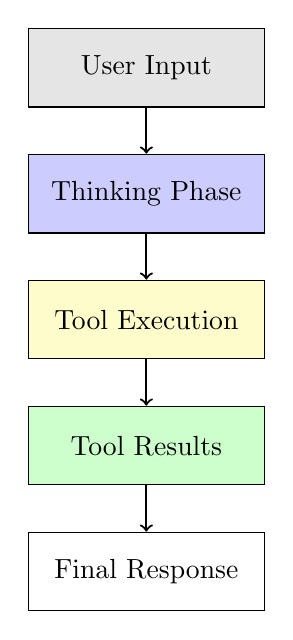
\begin{tikzpicture}[scale=0.8]
\node[rectangle, draw, fill=gray!20, minimum width=3cm, minimum height=1cm] (user) at (0,4) {User Input};
\node[rectangle, draw, fill=blue!20, minimum width=3cm, minimum height=1cm] (think) at (0,2) {Thinking Phase};
\node[rectangle, draw, fill=yellow!20, minimum width=3cm, minimum height=1cm] (tool) at (0,0) {Tool Execution};
\node[rectangle, draw, fill=green!20, minimum width=3cm, minimum height=1cm] (result) at (0,-2) {Tool Results};
\node[rectangle, draw, fill=white!20, minimum width=3cm, minimum height=1cm] (response) at (0,-4) {Final Response};

\draw[->, thick] (user) -- (think);
\draw[->, thick] (think) -- (tool);
\draw[->, thick] (tool) -- (result);
\draw[->, thick] (result) -- (response);
\end{tikzpicture}
\end{center}

\subsection{Streaming Implementation}

\begin{lstlisting}[caption=Streaming Chunk Processing]
CHUNK_TYPES = {
    "thinking": "Internal reasoning process",
    "tool_call": "Tool execution initiation",
    "tool_result": "Tool execution completion",
    "content": "Final response content",
    "error": "Error notifications"
}

def chat_stream(self, message: str, use_tools: bool = True):
    """Streaming chat with visual feedback."""
    for chunk in self._process_stream(message):
        chunk_type = chunk.get("type")
        content = chunk.get("content", "")

        if chunk_type == "thinking":
            # Gray text for internal reasoning
            print(f"\\033[90m{content}\\033[0m", end="", flush=True)
            yield {"type": "thinking", "content": content}

        elif chunk_type == "tool_call":
            # Blue notification for tool execution
            print(f"Tool: {content['name']}")
            yield {"type": "tool_call", "content": content}

        elif chunk_type == "tool_result":
            # Green result display
            print(f"Result: {content}")
            yield {"type": "tool_result", "content": content}

        elif chunk_type == "content":
            # Standard text for final response
            print(content, end="", flush=True)
            yield {"type": "content", "content": content}
\end{lstlisting}

\subsection{Performance Optimization}

The streaming system includes several optimization strategies:

\begin{itemize}
    \item \textbf{Chunk Batching}: Groups related content to reduce overhead
    \item \textbf{Buffer Management}: Intelligent buffering for smooth streaming
    \item \textbf{Backpressure Handling}: Prevents overwhelming the client with too many chunks
    \item \textbf{Timeout Protection}: Ensures streaming doesn't hang indefinitely
\end{itemize}

\section{Cross-Platform Compatibility}

\subsection{Platform Detection Strategy}

Intelligent platform detection with capability assessment:

\begin{lstlisting}[caption=Platform Detection Implementation]
def check_system_compatibility():
    """Comprehensive platform and capability detection."""
    system = platform.system()

    # macOS Detection
    if system == "Darwin":
        # Check for Apple Silicon vs Intel
        if platform.machine() == "arm64":
            return "ollama", "Apple Silicon Mac (M1/M2)"
        else:
            return "ollama", "Intel Mac"

    # Windows/Linux CUDA Detection
    if torch.cuda.is_available():
        gpu_name = torch.cuda.get_device_name(0)
        gpu_memory = torch.cuda.get_device_properties(0).total_memory

        if gpu_memory >= 4 * 1024**3:  # 4GB minimum
            return "vllm", f"NVIDIA GPU: {gpu_name} ({gpu_memory//1024**3}GB)"

    # CPU-based fallback
    cpu_count = multiprocessing.cpu_count()
    memory = psutil.virtual_memory().total

    return "ollama", f"CPU system ({cpu_count} cores, {memory//1024**3}GB RAM)"
\end{lstlisting}

\subsection{Backend Abstraction}

Unified interface across different backends:

\begin{lstlisting}[caption=Backend Abstraction Interface]
from abc import ABC, abstractmethod

class BaseAgent(ABC):
    """Abstract base class for all backend implementations."""

    @abstractmethod
    def chat(self, message: str, use_tools: bool = True,
             stream: bool = False) -> Union[str, Generator]:
        """Process a chat message with optional tool usage."""
        pass

    @abstractmethod
    def reset_conversation(self) -> None:
        """Reset conversation history."""
        pass

    @abstractmethod
    def get_system_info(self) -> Dict[str, Any]:
        """Get system and model information."""
        pass

class VLLMAgent(BaseAgent):
    """vLLM-specific implementation with GPU acceleration."""

    def __init__(self, model_name: str, host: str, port: int):
        self.model_name = model_name
        self.server = VLLMServer(host, port)
        self.client = OpenAI(base_url=f"http://{host}:{port}/v1")

    def chat(self, message: str, use_tools: bool = True,
             stream: bool = False):
        # vLLM-specific implementation
        pass

class OllamaAgent(BaseAgent):
    """Ollama implementation for local CPU inference."""

    def __init__(self, model_name: str):
        self.model_name = model_name
        self.client = ollama.Client()

    def chat(self, message: str, use_tools: bool = True,
             stream: bool = False):
        # Ollama-specific implementation
        pass
\end{lstlisting}

\subsection{Platform-Specific Setup}

\subsubsection{macOS Setup}

\begin{lstlisting}[caption=macOS Installation]
# Install via Homebrew
brew install ollama

# Start Ollama service
ollama serve  # Run in separate terminal

# Download default model
ollama pull qwen3:0.6b
\end{lstlisting}

\subsubsection{Windows Setup}

\begin{lstlisting}[caption=Windows Installation]
# Download from official website
# https://ollama.com/download/windows

# Install and start service
# Ollama will run as system service

# Download model via command line
ollama pull qwen3:0.6b
\end{lstlisting}

\subsubsection{Linux Setup}

\begin{lstlisting}[caption=Linux Installation]
# Install Ollama
curl -fsSL https://ollama.com/install.sh | sh

# Start service
sudo systemctl start ollama
sudo systemctl enable ollama

# Download model
ollama pull qwen3:0.6b

# For vLLM (requires CUDA)
# Install CUDA toolkit from NVIDIA
# vLLM will be automatically detected and used
\end{lstlisting}

\section{Testing and Development}

\subsection{Comprehensive Testing Framework}

The project includes extensive testing with multiple categories:

\begin{lstlisting}[caption=Test Structure]
tests/
|-- test_main.py              # Main agent functionality
|-- test_streaming.py         # Streaming implementation
|-- test_code_interpreter_full.py  # Tool execution testing
`-- conftest.py              # Test fixtures and mocks
\end{lstlisting}

\subsection{Unit Testing}

\begin{lstlisting}[caption=Backend Detection Testing]
def test_backend_detection():
    """Test automatic backend selection logic."""
    with patch('platform.system') as mock_system:
        with patch('torch.cuda.is_available') as mock_cuda:
            # Test macOS detection
            mock_system.return_value = "Darwin"
            backend, description = check_system_compatibility()
            assert backend == "ollama"
            assert "Mac" in description

            # Test Windows with CUDA
            mock_system.return_value = "Windows"
            mock_cuda.return_value = True
            backend, description = check_system_compatibility()
            assert backend == "vllm"
            assert "NVIDIA GPU" in description

            # Test Linux without CUDA
            mock_system.return_value = "Linux"
            mock_cuda.return_value = False
            backend, description = check_system_compatibility()
            assert backend == "ollama"
\end{lstlisting}

\subsection{Integration Testing}

\begin{lstlisting}[caption=Tool Execution Integration Test]
def test_tool_execution_workflow():
    """Test complete tool execution workflow."""
    agent = ToolCallingAgent(backend="ollama")

    # Test weather tool execution
    response = agent.chat("What's the weather in Tokyo?")

    # Verify response contains weather information
    assert "temperature" in response.lower() or "weather" in response.lower()
    assert "Tokyo" in response

    # Test code interpreter
    response = agent.chat("Calculate 2 + 2")
    assert "4" in response
\end{lstlisting}

\subsection{Mock-Based Testing}

\begin{lstlisting}[caption=Mock Testing Strategy]
def test_error_handling():
    """Test error propagation and formatting."""
    registry = ToolRegistry()

    # Test tool not found
    result = registry.execute_tool("nonexistent_tool", {})
    result_dict = json.loads(result)
    assert result_dict["success"] == False
    assert "not found" in result_dict["error"]

    # Test execution error
    result = registry.execute_tool("code_interpreter",
                                  {"code": "1/0"})
    result_dict = json.loads(result)
    assert result_dict["success"] == False
    assert "ZeroDivisionError" in result_dict["error"]
    assert "traceback" in result_dict
\end{lstlisting}

\subsection{Modern Development Workflow}

\begin{lstlisting}[caption=Development Commands]
# Install dependencies with UV
uv sync

# Run all tests
uv run pytest

# Run specific test file with verbose output
uv run pytest tests/test_main.py -v

# Run tests with coverage reporting
uv run pytest tests/ --cov=src/local_llm_serving

# Run single test by name pattern
uv run pytest -k "test_tool_execution"

# Format code with black
uv run black src/ tests/

# Sort imports with isort
uv run isort src/ tests/
\end{lstlisting}

\section{Configuration Management}

\subsection{Environment-Based Configuration}

\begin{lstlisting}[caption=Configuration Management]
# Load environment variables
from dotenv import load_dotenv
load_dotenv()

# Configuration with defaults
class Config:
    MODEL_NAME = os.getenv("MODEL_NAME", "Qwen/Qwen3-0.6B")
    VLLM_HOST = os.getenv("VLLM_HOST", "localhost")
    VLLM_PORT = int(os.getenv("VLLM_PORT", "8000"))
    LOG_LEVEL = os.getenv("LOG_LEVEL", "INFO")
    MAX_ITERATIONS = int(os.getenv("MAX_ITERATIONS", "10"))
    TOOL_TIMEOUT = int(os.getenv("TOOL_TIMEOUT", "30"))

    # Backend-specific settings
    OLLAMA_HOST = os.getenv("OLLAMA_HOST", "localhost")
    OLLAMA_PORT = int(os.getenv("OLLAMA_PORT", "11434"))
\end{lstlisting}

\subsection{Logging Configuration}

\begin{lstlisting}[caption=Logging Setup]
import logging
import sys

# Configure logging
logging.basicConfig(
    level=getattr(logging, Config.LOG_LEVEL),
    format='%(asctime)s - %(name)s - %(levelname)s - %(message)s',
    handlers=[
        logging.StreamHandler(sys.stdout),
        logging.FileHandler('logs/agent.log')
    ]
)

# Module-specific loggers
logger = logging.getLogger(__name__)
\end{lstlisting}

\section{Practical Exercises}

\subsection{Exercise 1: Custom Tool Development}

\textbf{Objective}: Implement a custom tool that integrates with an external API.

\textbf{Requirements}:
\begin{itemize}
    \item Create a tool that fetches current cryptocurrency prices
    \item Implement proper error handling and rate limiting
    \item Follow OpenAI function calling format
    \item Add comprehensive unit tests
\end{itemize}

\textbf{Solution Template}:
\begin{lstlisting}[caption=Custom Tool Implementation]
def get_crypto_price(symbol: str, currency: str = "USD") -> str:
    """Get current cryptocurrency price."""
    # Implementation here
    pass

# Register the tool
registry.register_tool(
    name="get_crypto_price",
    function=get_crypto_price,
    description="Get current price of a cryptocurrency",
    parameters={
        "type": "object",
        "properties": {
            "symbol": {"type": "string", "description": "Crypto symbol (BTC, ETH, etc.)"},
            "currency": {"type": "string", "description": "Currency code (USD, EUR, etc.)"}
        },
        "required": ["symbol"]
    }
)
\end{lstlisting}

\subsection{Exercise 2: Backend Implementation}

\textbf{Objective}: Implement a new backend for a different LLM provider.

\textbf{Requirements}:
\begin{itemize}
    \item Create a backend for Hugging Face Transformers
    \item Implement the BaseAgent interface
    \item Support both streaming and non-streaming modes
    \item Add tool calling capabilities
    \item Write integration tests
\end{itemize}

\textbf{Implementation Guidelines}:
\begin{lstlisting}[caption=New Backend Template]
class HuggingFaceAgent(BaseAgent):
    """Hugging Face Transformers backend implementation."""

    def __init__(self, model_name: str, device: str = "auto"):
        self.model_name = model_name
        self.device = self._get_device(device)
        self.tokenizer = AutoTokenizer.from_pretrained(model_name)
        self.model = AutoModelForCausalLM.from_pretrained(model_name)
        self.model.to(self.device)

    def chat(self, message: str, use_tools: bool = True,
             stream: bool = False):
        # Implementation here
        pass
\end{lstlisting}

\subsection{Exercise 3: Cross-Platform Deployment}

\textbf{Objective}: Deploy the application on different platforms with automated setup.

\textbf{Requirements}:
\begin{itemize}
    \item Create Docker containers for different platforms
    \item Implement automated setup scripts
    \item Add health checks and monitoring
    \item Document deployment procedures
    \item Test on multiple cloud providers
\end{itemize}

\subsection{Exercise 4: Performance Optimization}

\textbf{Objective}: Optimize the streaming performance and reduce latency.

\textbf{Requirements}:
\begin{itemize}
    \item Implement chunk batching for reduced overhead
    \item Add buffer management for smooth streaming
    \item Optimize tool execution parallelism
    \item Add caching for frequently used tools
    \item Measure and document performance improvements
\end{itemize}

\section{Assessment Criteria}

\subsection{Learning Outcomes Assessment}

Students will be evaluated based on their ability to:

\begin{enumerate}[label=\Alph*.]
    \item \textbf{Architecture Understanding} (25\%)
    \begin{itemize}
        \item Explain the Universal Agent Pattern and its benefits
        \item Describe the backend selection strategy and rationale
        \item Identify and explain the design patterns used
    \end{itemize}

    \item \textbf{Implementation Skills} (35\%)
    \begin{itemize}
        \item Implement custom tools following best practices
        \item Create backend implementations with proper interfaces
        \item Handle errors gracefully with appropriate feedback
    \end{itemize}

    \item \textbf{Testing Proficiency} (20\%)
    \begin{itemize}
        \item Write comprehensive unit tests with good coverage
        \item Implement integration tests for complex workflows
        \item Use mocking strategies effectively
    \end{itemize}

    \item \textbf{Cross-Platform Development} (20\%)
    \begin{itemize}
        \item Deploy applications on different platforms
        \item Handle platform-specific requirements
        \item Document deployment procedures clearly
    \end{itemize}
\end{enumerate}

\subsection{Practical Project Assessment}

\textbf{Final Project}: Students must implement a complete AI agent application with:
\begin{itemize}
    \item Custom domain-specific tools (minimum 3 tools)
    \item Multi-backend support (minimum 2 backends)
    \item Comprehensive test suite (minimum 80\% coverage)
    \item Cross-platform deployment documentation
    \item Performance optimization and benchmarking
    \item User documentation and API reference
\end{itemize}

\section{Conclusion}

This lecture has covered the comprehensive architecture and implementation of the Universal Tool Calling Demo, demonstrating advanced concepts in:

\begin{itemize}
    \item Modern AI agent development with multi-backend support
    \item OpenAI-compatible tool calling with extensible architecture
    \item Real-time streaming with visual feedback systems
    \item Cross-platform compatibility and intelligent fallback strategies
    \item Production-ready testing and deployment practices
    \item Software engineering patterns in AI application development
\end{itemize}

The project serves as an excellent foundation for understanding how to build sophisticated AI applications that work reliably across diverse computing environments while maintaining high performance and user experience standards.

\subsection{Further Reading}

\begin{enumerate}
    \item OpenAI Function Calling Documentation: \url{https://platform.openai.com/docs/guides/function-calling}
    \item ReAct Paper: "ReAct: Synergizing Reasoning and Acting in Language Models"
    \item vLLM Documentation: \url{https://docs.vllm.ai/}
    \item Ollama Documentation: \url{https://ollama.com/}
    \item Python Packaging with pyproject.toml: \url{https://packaging.python.org/en/latest/guides/writing-pyproject-toml/}
\end{enumerate}

\end{document}